\section{مقدمه}
{
	\begin{figure}[b]
		\centering
		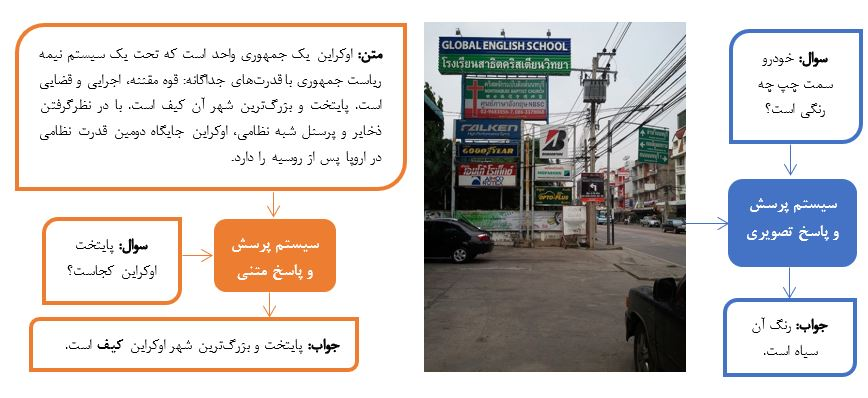
\includegraphics[scale=0.5]{images/vqa.JPG}
		\caption{مثالی از سیستم پرسش و پاسخ متنی و تصویری}
		\label{fig:8}
	\end{figure}

در طی سال‌های متمادی، محققان به دنبال ساخت ماشین‌هایی بودند که به اندازه‌ی کافی باهوش باشند که از آن به طور موثر همانند انسان‌ها برای تعامل استفاده کنند. مسئله‌ی پرسش و پاسخ تصویری یکی از پله‌های رسیدن به این رویای هوش مصنوعی است و از این جهت حائز اهمیت است. 

پرسش و پاسخ تصویری نسخه گسترش یافته مسئله پرسش و پاسخ متنی است که اطلاعات بصری به مسئله اضافه شده است. شکل
	\ref{fig:8}
 گویای تفاوت این دو مسئله است. در سیستم پرسش و پاسخ متنی، یک متن و یک سوال متنی به عنوان ورودی به سیستم داده می‌شود و انتظار می‌رود که سیستم با توجه به درک و تفسیری که از متن و سوال بدست می‌آورد؛ یک جواب متنی را خروجی دهد. اما در سیستم پرسش و پاسخ تصویری، یک تصویر و یک سوال متنی به ورودی سیستم داده می‌شود و انتظار می‌رود که سیستم بتواند با استفاده از عناصر بصری تصویر و تفسیری که از سوال بدست می‌آورد؛ یک پاسخ متنی را در خروجی نشان دهد. مسئله پرسش و پاسخ تصویری پیچیدگی بیشتری نسبت به مسئله پرسش و پاسخ متنی دارد زیرا تصاویر بعد بالاتر و نویز بیشتری نسبت به متن دارند. علاوه بر این، تصاویر فاقد ساختار و قواعد دستوری زبان هستند. در نهایت هم، تصاویر غنای بیشتری از دنیای واقعی را ضبط می‌کنند، در حالی که زبان طبیعی در حال حاضر نشانگر سطح بالاتری از انتزاع دنیای واقعی است
 	\cite{wu2017visual}.
 
 کاربردهای بسیاری برای پرسش و پاسخ تصویری وجود دارد. یکی از مهم‌ترین موارد دستیار هوشمند برای افراد کم‌بینا و نابینا 
 	\footnote{https://vizwiz.org/}
 است
 	\cite{gurari2018vizwiz}.
 علاوه بر این، در سال‌های اخیر دستیاران صوتی
 	\footnote{\lr{Voice Assistant}}
  و عامل‌های گفتگو 
  	\footnote{\lr{Conversational Agents}}
  مانند Siri ، Cortana و Alexa در بازار عرضه شدند که می‌توانند با انسان‌ها با استفاده از زبان طبیعی ارتباط برقرار کنند. در حال حاضر این دستیاران با استفاده از صوت و متن این ارتباط را برقرار می‌کنند در نتیجه گفتگوی بین این دستیاران با انسان‌ها مشابه دنیای واقعی نمی‌باشد. این ارتباط را می‌توان با استفاده از داده‌های تصویری و ویدئویی به واقعیت نزدیک‌تر کرد. اینجاست که مسئله‌ی پرسش و پاسخ تصویری برای نزدیک کردن تعامل بین انسان و عامل‌های گفتگو به دنیای واقعی می‌تواند موثر باشد. همین موضوع را می‌توانیم به صورت گسترده‌تری در ربات‌ها مشاهده کنیم. برای این‌که ربات بتواند بهتر با انسان‌ها ارتباط برقرار کند و به سوالات و درخواست‌ها پاسخ دهد؛ نیاز دارد که درک و فهم درستی از اطراف داشته باشد که این مستلزم داشتن تصویری دقیق از پیرامون است. بنابراین این ربات می‌تواند برای پاسخ به پرسش‌ها از دانشی که از طریق تصویر پیرامون خود بدست می‌آورد، جواب درستی را بدهد. کاربرد دیگر این مسئله در پزشکی است. در بسیاری موارد تحلیل تصاویر پزشکی مانند تصاویر CT‌ اسکن و x-ray برای یک پزشک متخصص هم دشوار است. اما یک سیستم پرسش و پاسخ تصویری می تواند با تحلیل و تشخیص موارد غیرطبیعی موجود در تصویر، به عنوان نظر دوم به پزشک متخصص کمک کند. از طرفی ممکن است در بعضی اوقات بیمار دسترسی به پزشک را نداشته باشد تا شرح تصاویر را متوجه شود. وجود سیستم پرسش و پاسخ تصویری می‌تواند آگاهی بیمار را نسبت به بیماری افزایش دهد و از نگرانی او بکاهد.
}